\documentclass[11pt]{article}
\usepackage[utf8]{inputenc}
\usepackage{amsmath}
\usepackage{amssymb}
\usepackage{graphicx}
\usepackage{hyperref}
\usepackage[parfill]{parskip}
\let\oldemptyset\emptyset
\let\emptyset\varnothing


\title{\textbf{Esssentials of Applied Data Analysis\\
				IPSA-USP Summer School 2017}\newline\\
				Central Limit Theorem}

\author{Leonardo Sangali Barone\\ \href{leonardo.barone@usp.br}{leonardo.barone@usp.br}}
\date{jan/17}

\begin{document}

\maketitle

\section*{Central Limit Theorem Simulation (PNUD 2010 HDI Data)}

There are 5565 municipalities in Brazil. PNUD uses data from the Brazilian Census to calculate the Human Development Index for each municipality. The data can be found at: http://www.pnud.org.br/atlas/ranking/ranking-idhm-municipios-2010.aspx\\

The mean HDI (Human Development Index) for Brazilian Muncipalities is $\mu_{HDI}=0.665$ and the standard deviation $\sigma_{HDI} = 0.072$.

	The HDI for all the municipalities is distributed as in Figure~\ref{f1}

\begin{figure}[htp]
\centering
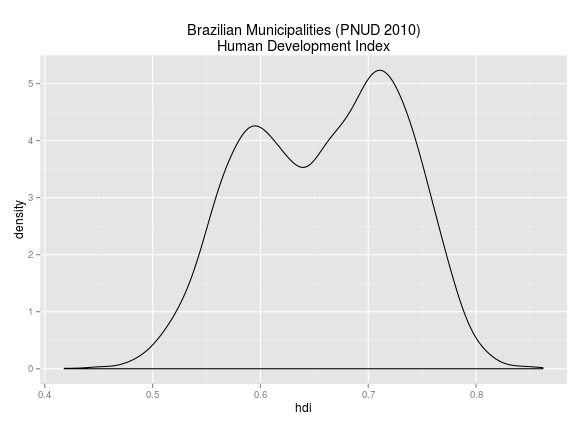
\includegraphics[scale=0.50]{clt_pop_dist.png}
\caption{Brazilian Municipalities Human Development Index (PNUD 2010)}
\label{f1}
\end{figure}

\subsection*{HDI in Brazilian Municipalities - 3 samples of different sizes}
	Let's now randomly draw 3 different samples, with 3 different sizes:\\

\begin{tabular}{|c|c|c|c|}
\hline
	Sample & $n_i$ & $\bar{x}_i$ & $\hat{\sigma}_i$\\
\hline
	1 & 36 & 0.644 & 0.071\\
	2 & 100 & 0.659 & 0.069\\
	3 & 1,600 & 0.658 & 0.071\\
\hline
\end{tabular}

Look at the distributions of the HDI in the 3 samples in Figure~\ref{f2}

\begin{figure}[htp]
\centering
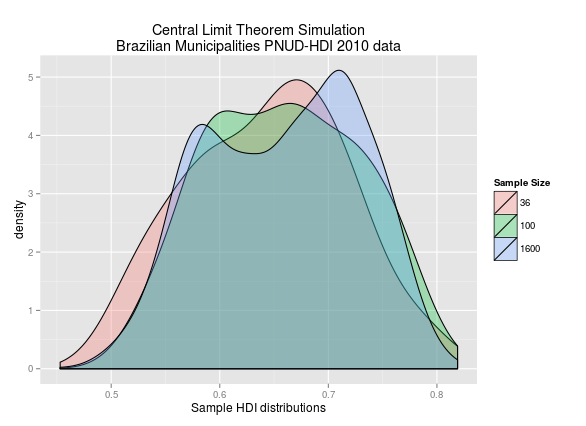
\includegraphics[scale=0.50]{clt_sample_dist.png}
\caption{}
\label{f2}
\end{figure}

	The distribution of HDI in the samples, as expected, resembles the distribution of HDI in the population of municipalities.\\

	Shouldn't it be normal? NO! Let' s take a look at the Central Limit Theorem!\\

	Remember: the distribution of the sample mean (of one characteristic of the population) is different from the distribution of the characteristic in the sample.

	\subsection*{Central Limit Theorem}
	Let $X_1,X_2,X_3,...$ be independent random variables identically distributed (all of the have the same probability function) with mean $\mu$ and variance $\sigma^2$ finite. Then if
	\[S= X_1 + X_2 + X_3 +...\]
	then S is a variable that is assimptoticaly (in the infinity!) normal.

	In other words, if there is a variable $S$ that is the sum of several independent variables with the same distribuition (like the mean of several sample means), then $S$ tend to be normal as the number of added variable grows.\\
	
	It is fundamental to notice that the $X_i$ variables (which is the variable in a single draw) does not need to be necessarely normal!

	\subsection*{Random Sample}
	A simple random sample of n subjects from a population is  one in which each possible sample of that size has the same probability (chance) of being selected.\\

For the CLT to hold (the sampling distribution and its standard error are as advertised), we must have a random  sample.

	\subsection*{Sample distribution of a parameter - HDI (2010)}
Going back to our example, even if we had only one sample, we would know how the sample mean is distributed (normally!) and we can calculated the standard deviation of that distribution (or standard error).\\

If, for example, we take a random sample of 100 municipalities and observe the sample mean ($\bar{x}$) what is the standard deviation of the sample mean ($\sigma_{\bar{x}}$)?

\[\sigma_{\bar{x}} = \frac{\sigma_{IDH}}{\sqrt{n}} = \frac{0.072}{\sqrt{100}} = \frac{0.072}{10} = 0.0072\]

	Now let's take 99,999 samples of size $n=36$, store the sample mean of each sample and plot the distribution. Let's repeat the proccess with sample with size $n=100$ and $n=1,600$. Check the result in Figure~\ref{f3}

	\begin{figure}[htp]
\centering
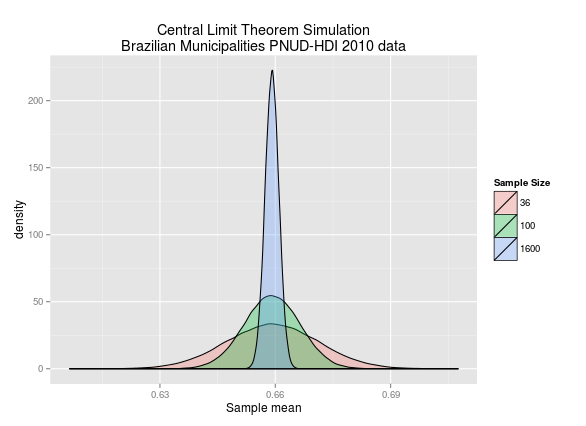
\includegraphics[scale=0.50]{clt_xbar_dist.png}
\caption{}
\label{f3}
\end{figure}

	All of them look a lot like normal curves (remember that we got that empirically by taking a lot of samples, not theoretically!).
	\newline\\
	By comparing the curves, can you guess the effect of the sample size when we build confidence intervals and hypothesis tests?	
\[\sigma_{\bar{x}} = \frac{\sigma_{IDH}}{\sqrt{n}}\]





\end{document}
